\documentclass[12pt,aspectratio=169,professionalfonts]{beamer}

\usepackage[T1]{fontenc}
\usepackage[utf8]{inputenc}
\usepackage{mathpazo}
\usepackage{amsmath}
\usepackage{graphicx}
\usepackage{tikz}
\usetikzlibrary{arrows.meta,calc,positioning,decorations.pathmorphing,shadows}

\usefonttheme{serif}

\definecolor{deepgreen}{HTML}{1E587A}
\definecolor{midgreen}{HTML}{AFCFE4}
\definecolor{softgreen}{HTML}{EAF4FA}
\definecolor{softline}{HTML}{C9DFEC}
\definecolor{darktext}{HTML}{111111}

\setbeamertemplate{navigation symbols}{}
\setbeamercolor{normal text}{fg=darktext,bg=white}
\setbeamercolor{frametitle}{fg=deepgreen,bg=softgreen}
\setbeamercolor{title}{fg=deepgreen}
\setbeamercolor{subtitle}{fg=deepgreen}
\setbeamercolor{structure}{fg=deepgreen}
\setbeamercolor{itemize item}{fg=darktext}
\setbeamercolor{itemize subitem}{fg=darktext}
\setbeamercolor{block title}{fg=deepgreen,bg=softgreen}
\setbeamercolor{block body}{fg=darktext,bg=white}
\setbeamercolor{author in head/foot}{fg=white,bg=deepgreen}
\setbeamercolor{title in head/foot}{fg=deepgreen,bg=midgreen}
\setbeamercolor{date in head/foot}{fg=deepgreen,bg=softgreen}

\setbeamertemplate{frametitle}{
  \nointerlineskip
  \begin{beamercolorbox}[wd=\paperwidth,ht=3.3ex,dp=1.2ex,leftskip=0.45cm,rightskip=0.2cm]{frametitle}
    \usebeamerfont{frametitle}\insertframetitle
  \end{beamercolorbox}
}

\setbeamertemplate{footline}{
  \leavevmode
  \hbox{
    \begin{beamercolorbox}[wd=.24\paperwidth,ht=2.8ex,dp=1.1ex,center]{author in head/foot}
      \scriptsize\insertshortauthor
    \end{beamercolorbox}
    \begin{beamercolorbox}[wd=.35\paperwidth,ht=2.8ex,dp=1.1ex,center]{title in head/foot}
      \scriptsize\insertshorttitle
    \end{beamercolorbox}
    \begin{beamercolorbox}[wd=.29\paperwidth,ht=2.8ex,dp=1.1ex,center]{date in head/foot}
      \scriptsize\insertshortdate
    \end{beamercolorbox}
    \begin{beamercolorbox}[wd=.12\paperwidth,ht=2.8ex,dp=1.1ex,rightskip=0.25cm]{date in head/foot}
      \scriptsize\insertframenumber/\inserttotalframenumber
    \end{beamercolorbox}
  }
}

\setbeamerfont{title}{size=\huge,series=\mdseries,shape=\itshape}
\setbeamerfont{subtitle}{size=\Large}
\setbeamerfont{frametitle}{size=\LARGE}
\setbeamerfont{itemize/enumerate body}{size=\normalsize}
\setbeamerfont{block title}{size=\normalsize}
\setbeamerfont{block body}{size=\normalsize}

\title[Wave Reconstruction]{How much information is needed to reconstruct a wave?}
\subtitle{Sparse samples, Fourier intuition, and Schr\"odinger evolution}
\author[J. P. G. Ramos]{Jo\~ao Pedro Gon\c calves Ramos}
\institute{IMPA}
\date[April 2026]{April 2026}

\newcommand{\placeholder}[1]{{\color{deepgreen}\textit{#1}}}

\newcommand{\logofallback}{%
  
\begin{tikzpicture}[baseline=-0.45ex]
    \draw[rounded corners=1pt,softline,line width=0.5pt,fill=softgreen] (0,0) rectangle (0.56,0.56);
    \draw[softline,line width=0.45pt] (0.09,0.09) -- (0.47,0.47);
    \draw[softline,line width=0.45pt] (0.47,0.09) -- (0.09,0.47);
  \end{tikzpicture}%
}

\newcommand{\institutionlogo}[1]{%
  \ifstrequal{#1}{ufrj}{
\includegraphics[width=0.72cm,height=0.62cm,keepaspectratio]{logos/ufrj-slide.png}}{%
  \ifstrequal{#1}{impa}{
\includegraphics[width=0.88cm,height=0.46cm,keepaspectratio]{logos/impa-slide.png}}{%
  \ifstrequal{#1}{bonn}{
\includegraphics[width=0.98cm,height=0.38cm,keepaspectratio]{logos/bonn-slide.png}}{%
  \ifstrequal{#1}{eth}{
\includegraphics[width=1.18cm,height=0.32cm,keepaspectratio]{logos/eth-slide.png}}{%
  \ifstrequal{#1}{epfl}{
\includegraphics[width=0.92cm,height=0.25cm,keepaspectratio]{logos/epfl-slide.png}}{%
  \ifstrequal{#1}{ulisbon}{
\includegraphics[width=0.52cm,height=0.68cm,keepaspectratio]{logos/ulisbon-slide.png}}{%
    \logofallback
  }}}}}}%
}

\newcommand{\institutionlogobox}[1]{%
  \makebox[1.16cm][c]{\raisebox{0pt}[0.64cm][0.08cm]{\institutionlogo{#1}}}%
}

\newcommand{\institutionbadge}[2]{%
  \institutionlogobox{#1}\hspace{0.18em}#2%
}

\newcommand{\waveband}{
  \begin{tikzpicture}[remember picture,overlay]
    \draw[softline,line width=1pt]
      ([yshift=1.0cm]current page.south west)
      .. controls +(3.2,0.55) and +(-3.2,-0.55) ..
      ([yshift=1.0cm]current page.south east);
    \draw[midgreen,line width=0.8pt]
      ([yshift=1.35cm]current page.south west)
      .. controls +(2.6,0.35) and +(-2.6,-0.35) ..
      ([yshift=1.35cm]current page.south east);
  \end{tikzpicture}
}

\newcommand{\samplingfigure}{
  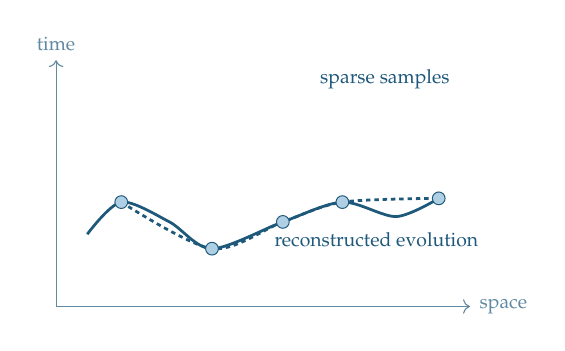
\begin{tikzpicture}[x=0.72cm,y=0.68cm]
    \draw[->,deepgreen!70] (0,0) -- (7.3,0) node[right] {\scriptsize space};
    \draw[->,deepgreen!70] (0,0) -- (0,4.6) node[above] {\scriptsize time};
    \draw[deepgreen,line width=1pt]
      plot[smooth] coordinates {
        (0.55,1.35) (1.15,1.95) (2.00,1.58) (2.75,1.08)
        (4.00,1.58) (5.05,1.95) (6.00,1.68) (6.75,2.02)
      };
    \draw[deepgreen,dash pattern=on 1.6pt off 1.4pt,line width=1pt]
      plot[smooth] coordinates {
        (1.15,1.95) (2.75,1.08) (4.00,1.58) (5.05,1.95) (6.75,2.02)
      };
    \foreach \p in {(1.15,1.95),(2.75,1.08),(4.00,1.58),(5.05,1.95),(6.75,2.02)} {
      \filldraw[deepgreen,line width=0.35pt,fill=midgreen] \p circle (2.3pt);
    }
    \node[deepgreen,align=center] at (5.8,4.25) {\scriptsize sparse samples};
    \node[deepgreen,align=center] at (5.65,1.25) {\scriptsize reconstructed evolution};
  \end{tikzpicture}
}

\newcommand{\motivationfigure}{
  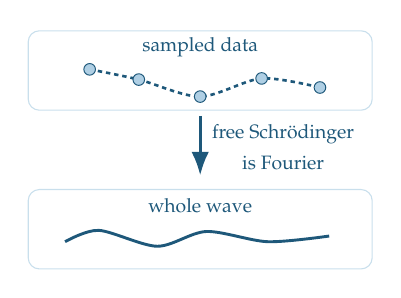
\begin{tikzpicture}[x=0.78cm,y=0.72cm]
    \draw[softline,rounded corners] (0.2,3.1) rectangle (5.8,4.5);
    \draw[softline,rounded corners] (0.2,0.3) rectangle (5.8,1.7);
    \draw[deepgreen,dash pattern=on 1.6pt off 1.4pt,line width=0.95pt]
      plot[smooth] coordinates {
        (1.20,3.82) (2.00,3.64) (3.00,3.34) (4.00,3.66) (4.95,3.50)
      };
    \foreach \p in {(1.20,3.82),(2.00,3.64),(3.00,3.34),(4.00,3.66),(4.95,3.50)} {
      \filldraw[deepgreen,line width=0.35pt,fill=midgreen] \p circle (2.1pt);
    }
    \node[deepgreen] at (3.0,4.22) {\scriptsize sampled data};
    \draw[-{Latex[length=3mm]},line width=1.05pt,deepgreen] (3.0,3.0) -- (3.0,1.95);
    \node[deepgreen,align=center] at (4.35,2.45) {\scriptsize free Schr\"odinger\\[-0.02cm]\scriptsize is Fourier};
    \draw[deepgreen,line width=1.05pt]
      plot[smooth] coordinates {
        (0.80,0.78) (1.35,0.98) (2.30,0.70) (3.10,0.96) (4.10,0.78) (5.10,0.88)
      };
    \node[deepgreen] at (3.0,1.42) {\scriptsize whole wave};
  \end{tikzpicture}
}

\newcommand{\researchfigure}{
  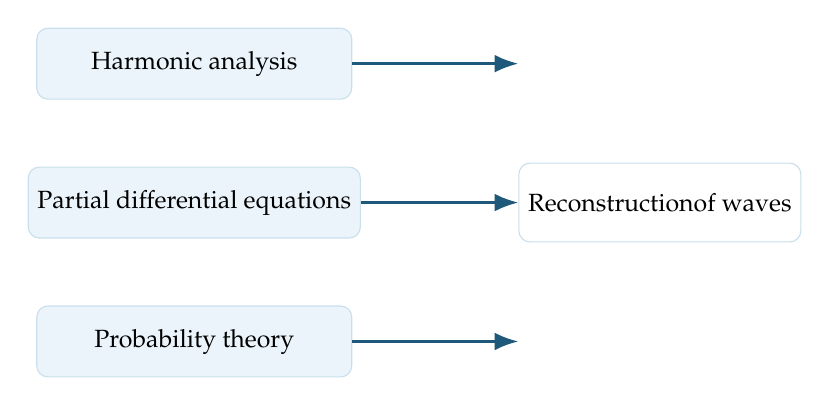
\begin{tikzpicture}[node distance=0.85cm]
    \node[draw=softline,rounded corners,fill=softgreen,minimum width=4.0cm,minimum height=0.9cm] (ha)
      {\small Harmonic analysis};
    \node[draw=softline,rounded corners,fill=softgreen,minimum width=4.0cm,minimum height=0.9cm,below=of ha] (pde)
      {\small Partial differential equations};
    \node[draw=softline,rounded corners,fill=softgreen,minimum width=4.0cm,minimum height=0.9cm,below=of pde] (prob)
      {\small Probability theory};
    \node[draw=softline,rounded corners,fill=white,minimum width=2.6cm,minimum height=1.0cm,right=2.0cm of pde] (goal)
      {\small Reconstruction\\[-0.05cm]\small of waves};
    \draw[-{Latex[length=3mm]},deepgreen,line width=1pt] (ha.east) -- (goal.west |- ha.east);
    \draw[-{Latex[length=3mm]},deepgreen,line width=1pt] (pde.east) -- (goal.west);
    \draw[-{Latex[length=3mm]},deepgreen,line width=1pt] (prob.east) -- (goal.west |- prob.east);
  \end{tikzpicture}
}

\newcommand{\transferfigure}{
  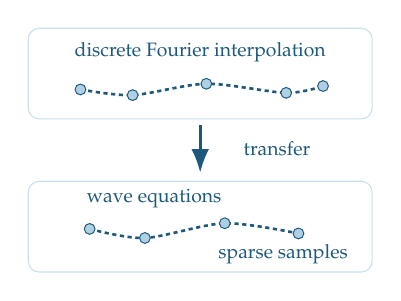
\begin{tikzpicture}[x=0.78cm,y=0.72cm]
    \draw[softline,rounded corners] (0.2,3.0) rectangle (5.8,4.6);
    \draw[softline,rounded corners] (0.2,0.3) rectangle (5.8,1.9);
    \node[deepgreen] at (3.0,4.18) {\scriptsize discrete Fourier interpolation};
    \draw[deepgreen,dash pattern=on 1.5pt off 1.3pt,line width=0.95pt]
      plot[smooth] coordinates {
        (1.05,3.52) (1.90,3.42) (3.10,3.62) (4.40,3.46) (5.00,3.58)
      };
    \foreach \p in {(1.05,3.52),(1.90,3.42),(3.10,3.62),(4.40,3.46),(5.00,3.58)} {
      \filldraw[deepgreen,line width=0.35pt,fill=midgreen] \p circle (1.95pt);
    }
    \draw[-{Latex[length=3mm]},line width=1.05pt,deepgreen] (3.0,2.9) -- (3.0,2.05);
    \node[deepgreen] at (4.25,2.48) {\scriptsize transfer};
    \node[deepgreen] at (2.25,1.60) {\scriptsize wave equations};
    \draw[deepgreen,dash pattern=on 1.5pt off 1.3pt,line width=0.95pt]
      plot[smooth] coordinates {
        (1.20,1.06) (2.10,0.90) (3.40,1.16) (4.60,0.98)
      };
    \foreach \p in {(1.20,1.06),(2.10,0.90),(3.40,1.16),(4.60,0.98)} {
      \filldraw[deepgreen,line width=0.35pt,fill=midgreen] \p circle (1.95pt);
    }
    \node[deepgreen] at (4.35,0.62) {\scriptsize sparse samples};
  \end{tikzpicture}
}

\newcommand{\conjecturefigure}{
  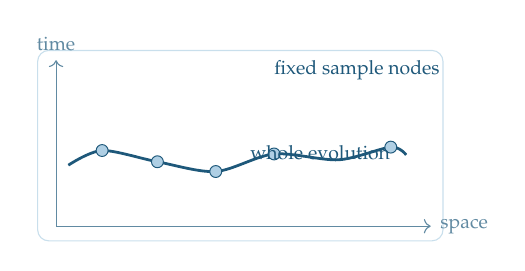
\begin{tikzpicture}[x=0.78cm,y=0.62cm]
    \draw[softline,rounded corners] (0.2,0.5) rectangle (6.8,4.4);
    \draw[->,deepgreen!70] (0.5,0.8) -- (6.6,0.8) node[right] {\scriptsize space};
    \draw[->,deepgreen!70] (0.5,0.8) -- (0.5,4.2) node[above] {\scriptsize time};
    \draw[deepgreen,line width=1pt]
      plot[smooth] coordinates {
        (0.70,2.05) (1.25,2.35) (2.15,2.12) (3.10,1.92)
        (4.05,2.28) (5.10,2.16) (5.95,2.42) (6.20,2.26)
      };
    \foreach \p in {(1.25,2.35),(2.15,2.12),(3.10,1.92),(4.05,2.28),(5.95,2.42)} {
      \filldraw[deepgreen,line width=0.35pt,fill=midgreen] \p circle (2.15pt);
    }
    \node[deepgreen,align=center] at (5.4,4.0) {\scriptsize fixed sample nodes};
    \node[deepgreen,align=center] at (4.8,2.3) {\scriptsize whole evolution};
  \end{tikzpicture}
}

\begin{document}

\begin{frame}[plain]
  \begin{tikzpicture}[remember picture,overlay]
    \node[
      name=titlepanel,
      rounded corners=8pt,
      fill=softgreen,
      drop shadow={shadow xshift=0.9ex,shadow yshift=-0.6ex,opacity=0.35},
      minimum width=0.93\paperwidth,
      minimum height=2.25cm,
      anchor=north
    ] at ([yshift=-1.2cm]current page.north) {};
    \node[anchor=center,text width=0.84\paperwidth,align=center,text=deepgreen]
      at ([yshift=0.12cm]titlepanel.center)
      {\usebeamerfont{title}\inserttitle};
    \draw[midgreen,line width=1pt]
      ([xshift=-4.8cm,yshift=1.2cm]current page.south)
      .. controls +(1.7,0.45) and +(-1.7,-0.45) ..
      ([xshift=4.8cm,yshift=1.2cm]current page.south);
  \end{tikzpicture}

  \vspace{3.2cm}
  \begin{center}
    {\Large Jo\~ao Pedro Gon\c calves Ramos\par}
    \vspace{0.45cm}
    {\large IMPA\par}
    \vspace{0.6cm}
    {\large April 2026\par}
  \end{center}
\end{frame}

\begin{frame}{My path so far}
  \waveband
  \vspace{0.05cm}
  \scriptsize
  \renewcommand{\arraystretch}{0.98}
  \begin{tabular}{@{}p{0.20\linewidth} p{0.39\linewidth} p{0.25\linewidth}@{}}
    \textbf{\color{deepgreen}2015--2016} &
      \institutionbadge{ufrj}{UFRJ} &
      Undergraduate
      \\[0.04cm]
    \textbf{\color{deepgreen}2014--2016} &
      \institutionbadge{impa}{IMPA} &
      Master's
      \\[0.04cm]
    \textbf{\color{deepgreen}2016--2020} &
      \institutionbadge{bonn}{Bonn} &
      PhD
      \\[0.04cm]
    \textbf{\color{deepgreen}2020--2024} &
      \institutionbadge{impa}{IMPA} &
      \\[-0.10cm]
    &
      \institutionbadge{eth}{ETH Z\"urich} &
      Postdocs
      \\[-0.10cm]
    &
      \institutionbadge{epfl}{EPFL} &
      \\[0.02cm]
    \textbf{\color{deepgreen}2024--2025} &
      \institutionbadge{ulisbon}{ULisbon} &
      Tenure-track
      \\[0.04cm]
    \textbf{\color{deepgreen}2025--current} &
      \institutionbadge{impa}{IMPA} &
      Current position
  \end{tabular}
\end{frame}

\begin{frame}{My work so far}
  \waveband
  \vspace{0.35cm}
  {\Large Harmonic analysis\par}
  \vspace{0.18cm}
  {\Large Partial differential equations\par}
  \vspace{0.18cm}
  {\Large Probability theory\par}
  \vspace{0.55cm}
  {\normalsize\color{deepgreen}Selected highlights\par}
  \vspace{0.15cm}
  {\large Concentration for STFT (\textit{Inventiones})\par}
  \vspace{0.12cm}
  {\large Interpolation formulas and Fourier uniqueness\par}
  \vspace{0.12cm}
  {\large Stability for sphere packings in dimensions 8 and 24\par}
\end{frame}

\begin{frame}{The big question}
  \waveband
  \vspace{0.25cm}
  \begin{columns}[T,totalwidth=\textwidth]
    \column{0.54\textwidth}
      {\Large\color{deepgreen}How much information determines a wave?\par}
      \vspace{0.2cm}
      \begin{itemize}[<+->]
        \item We almost never observe a whole system.
        \item We only see sparse samples in space and time.
        \item Can those samples determine the full evolution?
      \end{itemize}
    \column{0.42\textwidth}
      \vspace{0.2cm}
      \samplingfigure
  \end{columns}
\end{frame}

\begin{frame}{Why might samples be enough?}
  \waveband
  \vspace{0.35cm}
  \begin{columns}[T,totalwidth=\textwidth]
    \column{0.54\textwidth}
      \begin{itemize}[<+->]
        \item In Fourier analysis, discrete samples can determine a function.
        \item For the free Schr\"odinger equation, Fourier analysis writes the evolution explicitly.
        \item This suggests that sparse samples may determine the whole wave.
      \end{itemize}
      \vspace{0.6cm}
      \[
        i\partial_t u + \Delta u = 0
      \]
    \column{0.42\textwidth}
      \vspace{0.25cm}
      \motivationfigure
  \end{columns}
\end{frame}

\begin{frame}{Going deeper}
  \waveband
  \vspace{0.35cm}
  \begin{columns}[T,totalwidth=\textwidth]
    \column{0.56\textwidth}
      \begin{itemize}[<+->]
        \item Viazovska's sphere-packing breakthrough led to new Fourier interpolation formulas.
        \item Recent PDE results already translate Fourier intuition into rigidity for waves.
        \item Can sparse-sampling principles survive beyond the Fourier setting?
      \end{itemize}
      \vspace{0.35cm}
      {\normalsize\color{deepgreen}Names to mention orally: Viazovska; Radchenko and Viazovska.}
    \column{0.4\textwidth}
      \vspace{0.15cm}
      \transferfigure
  \end{columns}
\end{frame}

\begin{frame}{Main conjecture}
  \waveband
  \vspace{0.25cm}
  \begin{columns}[T,totalwidth=\textwidth]
    \column{0.55\textwidth}
      \begin{block}{}
        Fixed sparse samples in space and time can determine the whole wave.
      \end{block}
      \vspace{0.35cm}
      \begin{itemize}[<+->]
        \item Reconstruction from very limited sampled data.
        \item First in linear models.
        \item Then in nonlinear Schr\"odinger-type evolutions.
      \end{itemize}
    \column{0.41\textwidth}
      \vspace{0.25cm}
      \conjecturefigure
  \end{columns}
\end{frame}

\begin{frame}{Why this project stands out}
  \waveband
  \vspace{0.25cm}
  \begin{itemize}[<+->]
    \item \textbf{Boldness.} It asks for reconstruction well beyond the current Fourier formulas.
    \item \textbf{Originality.} It unifies harmonic analysis and dispersive PDE in a single framework.
    \item \textbf{Impact.} It changes how we think about partial observation of wave phenomena and opens a route toward algorithmic reconstruction.
    \item \textbf{Positioning.} My work sits on both sides of this bridge: Fourier uniqueness and dispersive PDE.
  \end{itemize}
\end{frame}

\begin{frame}[plain]
  \begin{tikzpicture}[remember picture,overlay]
    \draw[softline,line width=1pt]
      ([xshift=-5.2cm,yshift=1.45cm]current page.south)
      .. controls +(1.7,0.55) and +(-1.7,-0.55) ..
      ([xshift=5.2cm,yshift=1.45cm]current page.south);
    \draw[midgreen,line width=1pt]
      ([xshift=-5.2cm,yshift=1.85cm]current page.south)
      .. controls +(1.5,0.35) and +(-1.5,-0.35) ..
      ([xshift=5.2cm,yshift=1.85cm]current page.south);
    \foreach \x in {-4.3,-2.7,-1.0,0.8,2.4,4.0} {
      \fill[midgreen] ([xshift=\x cm,yshift=1.45cm]current page.south) circle (2pt);
    }
  \end{tikzpicture}
  \vspace{2.2cm}
  \begin{center}
    {\huge\color{deepgreen}Very little information may be enough to determine a wave.\par}
    \vspace{1cm}
    {\Large Thank you.\par}
  \end{center}
\end{frame}

\end{document}
